\documentclass[a4 paper]{article}
%\usepackage{minted}           %embedding code
\usepackage{amsmath, amsthm, amsfonts} %always use amsmath for symbols, amsthm for theorems 
\usepackage{graphicx}  % for pictures
%\usepackage{lipsum}  % for test text
\usepackage{multicol}    % for multicollumn text
\usepackage[bottom=2.5cm]{geometry}   %to set the margins to your liking
\usepackage[skip = 10pt, indent = 30pt]{parskip}      %to set the distance between paragraphs
\usepackage{tcolorbox}           %for literal color boxes
%\usepackage{witharrows}             % understandable, arrows for equations
\usepackage{tikz}                   %drawings and diagrams
\usetikzlibrary{positioning}        %tikz library for positioning (of nodes?)
\usepackage{pgfplots}               %plotting and graphs
\pgfplotsset{compat=1.18, width = 10cm}
\usepackage{hyperref}
\hypersetup{colorlinks = true, linkcolor = black, urlcolor = blue}
%\usepackage{fancyvrb}           % fancy formatting of verbatim
%\usepackage{fancyhdr, lastpage}
%\pagestyle{fancy} 
%\lhead{Relat\'orio experimento 4}
%\rhead{FisExpI}
%\cfoot{Página \thepage \ de \pageref{LastPage}}
%\usepackage[Bjornstrup]{fncychap} %Sonny, Glenn, Lenny, Conny, Rejne, Bjarne, Bjornstrup
%\usepackage{xcolor}      %color text
\usepackage{siunitx}    %for SI units
\usepackage{setspace}
\onehalfspacing
\usepackage{cleveref}
\usepackage[brazil]{babel}
\usepackage{caption}
\usepackage{subcaption}
\usepackage{pdfpages}
\usepackage{booktabs}
\usepackage{multirow}
\usepackage{textcomp}
\usepackage{amssymb}
\usepackage[document]{ragged2e}
\usepackage{bm}
\usepackage{empheq}




%\setlength{\hoffset}{-2cm}
%\setlength{\voffset}{1.5cm}                     %control your margins however you want!
%\setlength{\marginparwidth}{2cm}
%\setlength{\oddsidemargin}{0cm}

%\newtheorem{theorem}{Theorem}[section]               %how you call it and how you display it
%\newtheorem{corollary}{Corollary}[theorem]


\newcommand{\parag}{\hspace{30pt}}
%\newcommand{\pd}[2]{\frac{\partial#1}{\partial#2}}


\begin{document}


\justifying
\begin{center}{\large Laboratório de Circuitos Elétricos - 02/2024 - Turma 05}\\
{\large \textbf{Experimento 5}}\\ 
05/12/2024
\end{center}

\vspace{500pt}
 \noindent\textbf{Grupo 5:}\\
 Yuri Shumyatsky - 231012826\\
Vinicius de Melo Moraes - 231036274\\



\vspace{30pt}
\newpage

\section{Introdução}

\section{Materiais}


	\begin{itemize}
	\item National Instruments Elvis II
	\item 2 capacitor de 47n$F$
	\item 2 resistor de 1,2k$\Omega$
	
	\end{itemize}

\newpage

\section{Procedimento}

\parag O National Instruments Elvis é usado como fonte, protoboard, e multímetro. Usa-se a função de multímetro para checar as resistências e capacitâncias dos componentes, que são marcadas na Tabela 1.

\vspace{5pt}
\begin{table}[h]
\centering
\begin{tabular}{|c|c|c|c|}
\hline
\textbf{Grandeza} & \textbf{Valor nominal} & \textbf{Valor medido} & \textbf{Erro (\%)} \\\hline
$R_1$ & 1,2k$\Omega$ & 1,1718k$\Omega$ & 2,35\\\hline
$R_2$ & 1,2k$\Omega$ & 1,1810$\Omega$ & 1,58\\\hline
$C_1$ & 47nF & 49,90nF & 6,17\\\hline
$C_2$ & 47nF & 47,54nF & 1,15\\\hline
\end{tabular}
\caption*{Tabela 1: Componentes}
\end{table}

Em seguida, os componentes são usados para montar o circuito da Figura 1.

\begin{table}[h]
\centering
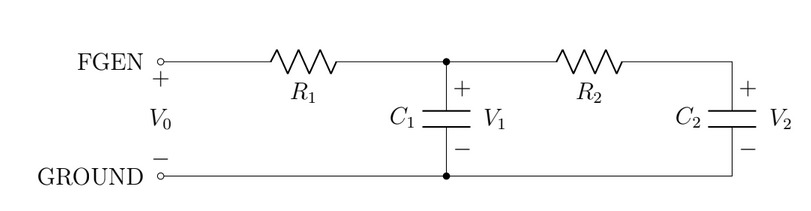
\includegraphics[scale=0.7]{figuras/figura1}
\end{table}

\begin{center}
Figura 1: Circuito em regime AC
\end{center}

O Elvis possui um gerador de funções, que é usado para produzir uma onda senoidal com $2V_{pp}$, offset zero e frequência de $250Hz$. Além do gerador, o equipamento também possui um osciloscópio, que é usado para medir as tensões relevantes e produzir os gráficos.

Para começar, é feita a transformação do circuito para o domínio dos fasores, de forma a facilitar as contas. Isso resulta no circuito da Figura 2.

\begin{table}[h]
\centering
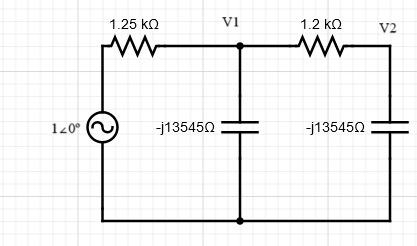
\includegraphics[scale=0.7]{figuras/figura2}
\end{table}

\begin{center}
Figura 2: Circuito no domínio fasorial
\end{center}

Nesse formato do circuito, foi feita análise nodal para obter as tensões $V_1$ e $V_2$.

\newpage
LKC nó 1:
\[\frac{(-1+V_1)}{1250}+\frac{V_1}{-j13545}+\frac{(-V_2+V_1)}{1200}=0\]

LKC nó 2:
\[-\frac{V_2}{j13545}-\frac{(-V_2+V_1)}{1200}=0\]
que simplificam no seguinte sistema:

\begin{equation*}
\left\{
\begin{aligned}
V_1(16,33+j0,74)-V_2(8,33)=8\\
V_1(-8,33)+V_2(8,33+j0,74)=0
\end{aligned}\right.
\end{equation*}

Com isso obtemos os valores esperados de $V_1=0,959-j0,175$ e $V_2=0,937-j0,259$, que podem ser transformados nas suas formas polares $V_1=0,975\angle(-10,34$\textdegree) e $V_2=0,972\angle(-15,45$\textdegree)

Seguem o os Gráficos 1 e 2 que demonstram a diferença de amplitude entre $V_0$ e $V_1$ e $V_0$ e $V_2$, respectivamente. Em azul escuro, temos a tensão da fonte e em verde as tensões capacitivas.

\begin{table}[h]
\centering
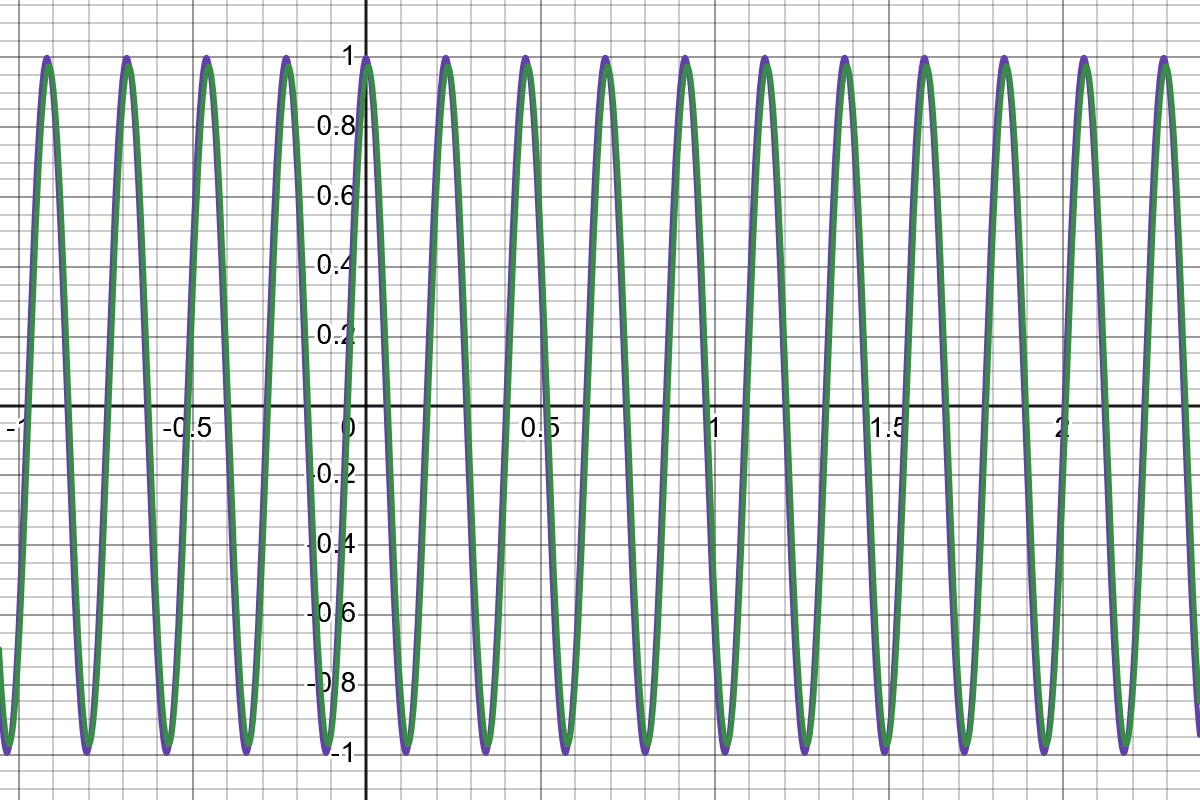
\includegraphics[scale=0.225]{rgadicoas/grafico1}
\end{table}

\begin{center}
Gráfico 1: Tensão da fonte e $V_1$
\end{center}


\begin{table}[h]
\centering
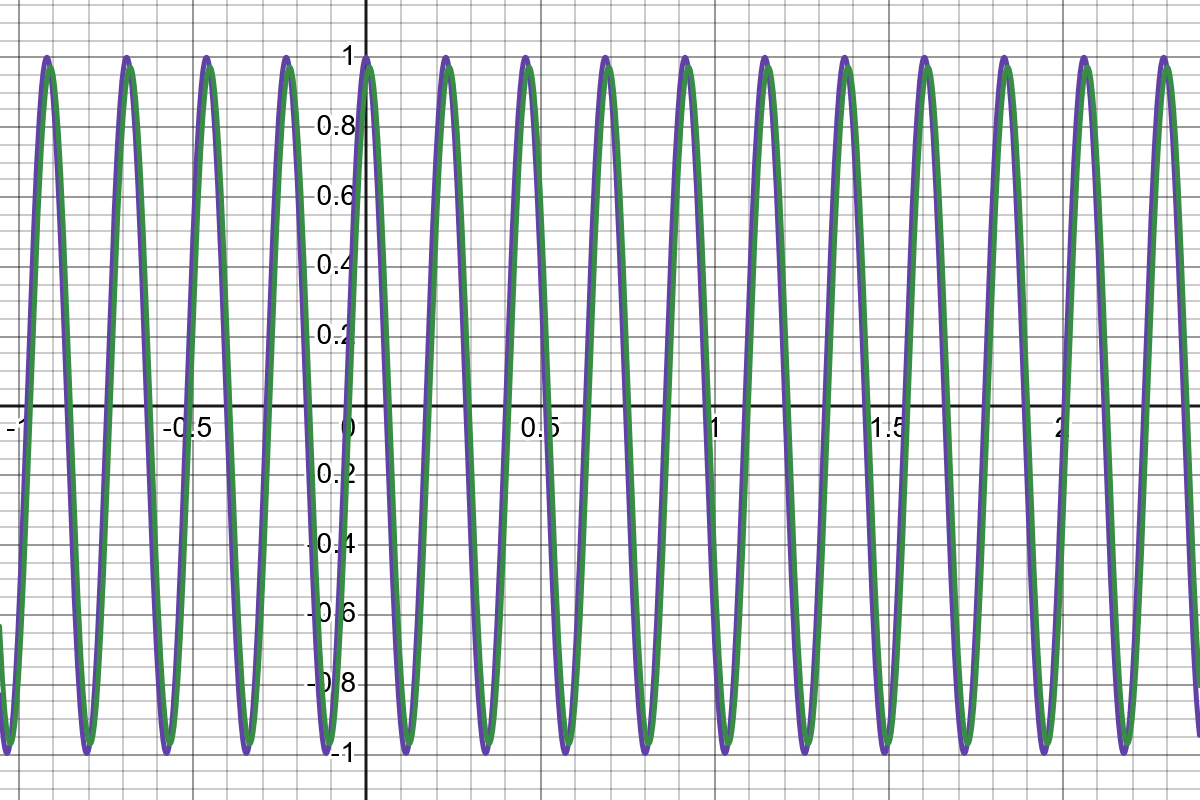
\includegraphics[scale=0.225]{rgadicoas/grafico5}
\end{table}

\begin{center}
Gráfico 2: Tensão da fonte e $V_2$
\end{center}

Em seguida, o processo é repetido para as frequências de $500Hz$, $1kHz$ e $2kHz$. Como a única parte alterada em todas contas é a impedância dos capacitores, que depende de $\omega$ (uma vez que $Z_c=\dfrac{1}{j\omega C}$), de forma análoga se encontram  os valores de $V_1$ e $V_2$ expostos a seguir, e seus gráficos.

\begin{table}[h]
\centering
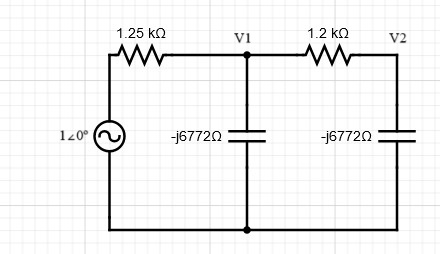
\includegraphics[scale=0.6]{figuras/figura3}
\end{table}

\begin{center}
Figura 3: Circuito no domínio fasorial para $\omega=1000\pi$
\end{center}

$f=500Hz\implies \omega = 1000\pi:$\\\centering
$V_1=0,859-j0,307 = 0,910\angle(-19,25$\textdegree)\\
$V_2=0,778-j0,447=0,897\angle(-29,88$\textdegree)\\
\justifying

\begin{table}[h]
\centering
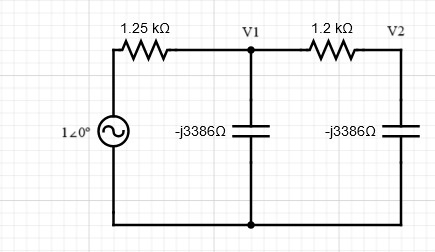
\includegraphics[scale=0.6]{figuras/figura4}
\end{table}

\begin{center}
Figura 4: Circuito no domínio fasorial para $\omega=2000\pi$
\end{center}

$f=1kHz\implies \omega = 2000\pi:$\\\centering
$V_1=0,639-j0,403=0,755\angle(-32,24$\textdegree)\\
$V_2=0,437-j0,561=0,711\angle(-52,08$\textdegree)\\
\justifying

\begin{table}[h]
\centering
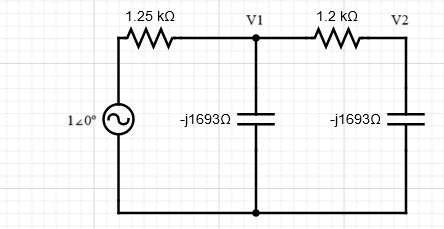
\includegraphics[scale=0.6]{figuras/figura5}
\end{table}

\begin{center}
Figura 5: Circuito no domínio fasorial para $\omega=4000\pi$
\end{center}

$f=2kHz\implies \omega = 4000\pi:$\\\centering
$V_1=0,401-j0,367=0,544\angle(-42,47$\textdegree)\\
$V_2=0,089-j0,432=0,441\angle(-78,36$\textdegree)\\
\justifying

\newpage
\begin{table}[h]
\centering
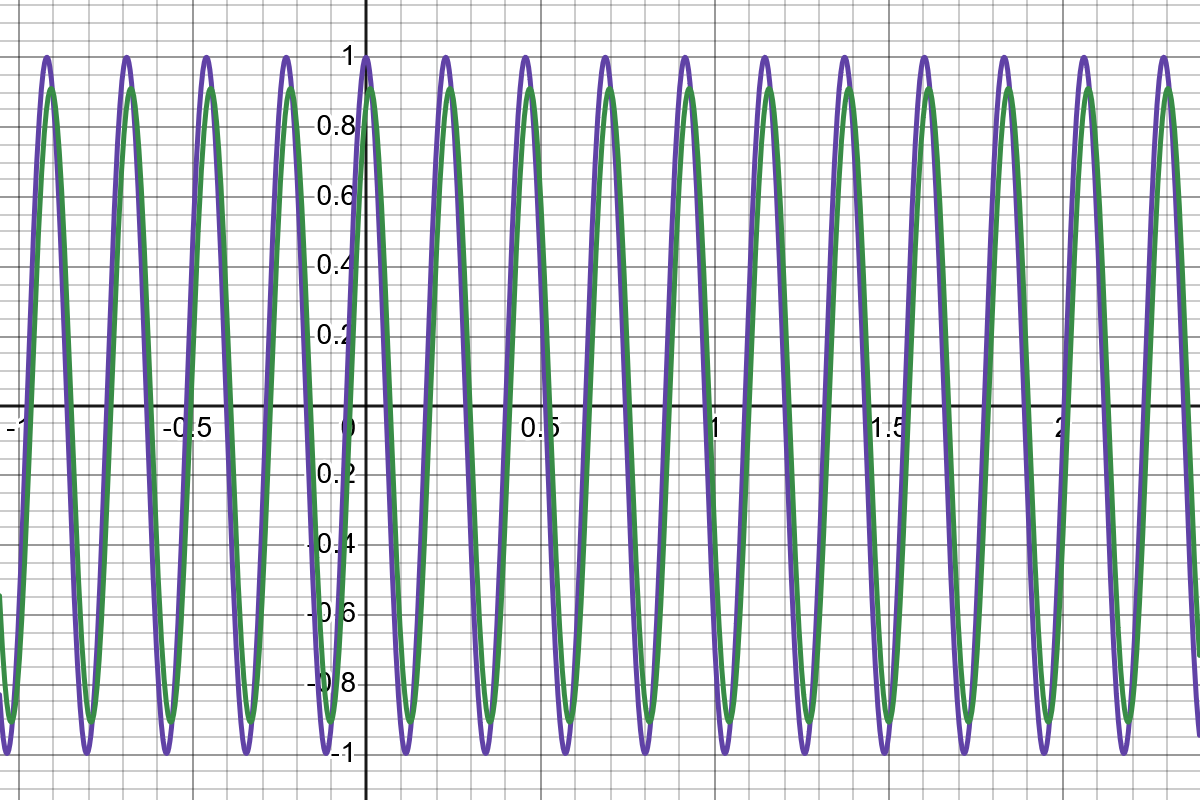
\includegraphics[scale=0.25]{rgadicoas/grafico2}
\end{table}

\begin{center}
Gráfico 3: Tensão da fonte e $V_1$ em $\omega =1000\pi$
\end{center}

\vspace{30pt}
\begin{table}[h]
\centering
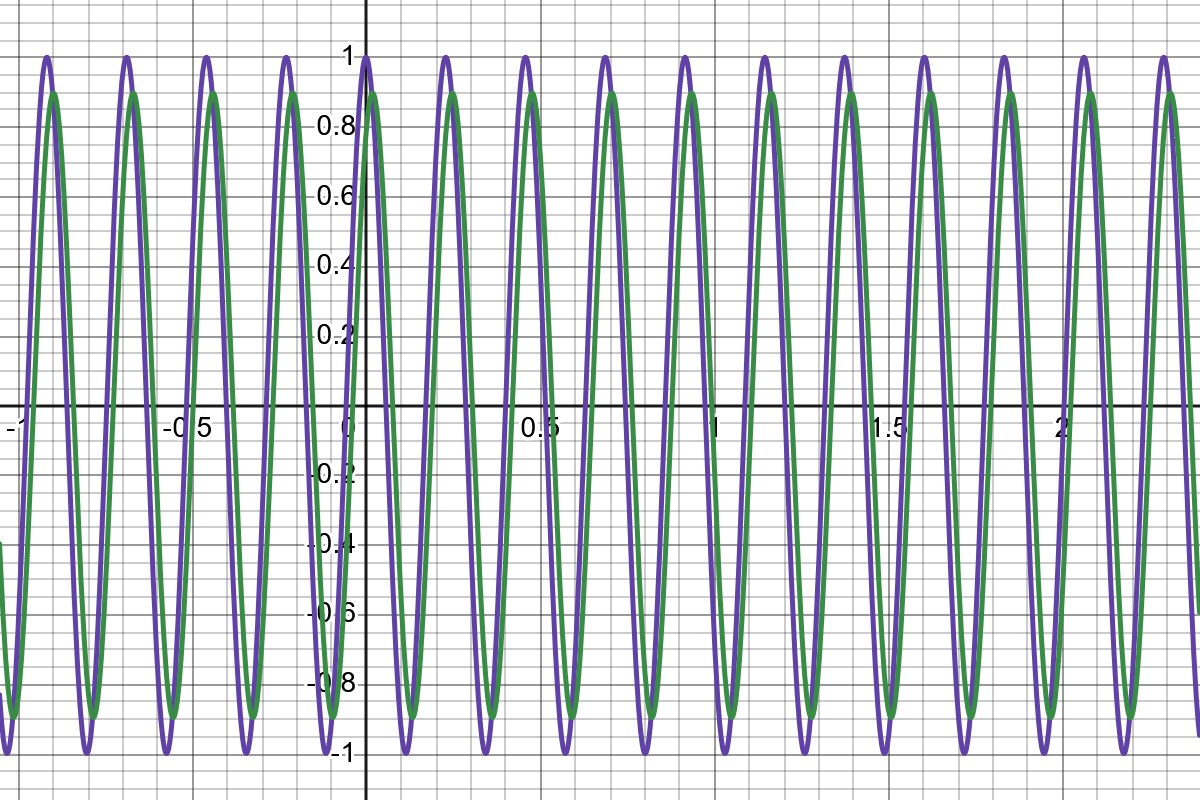
\includegraphics[scale=0.25]{rgadicoas/grafico6}
\end{table}

\begin{center}
Gráfico 4: Tensão da fonte e $V_2$ em $\omega =1000\pi$
\end{center}

\begin{table}[h]
\centering
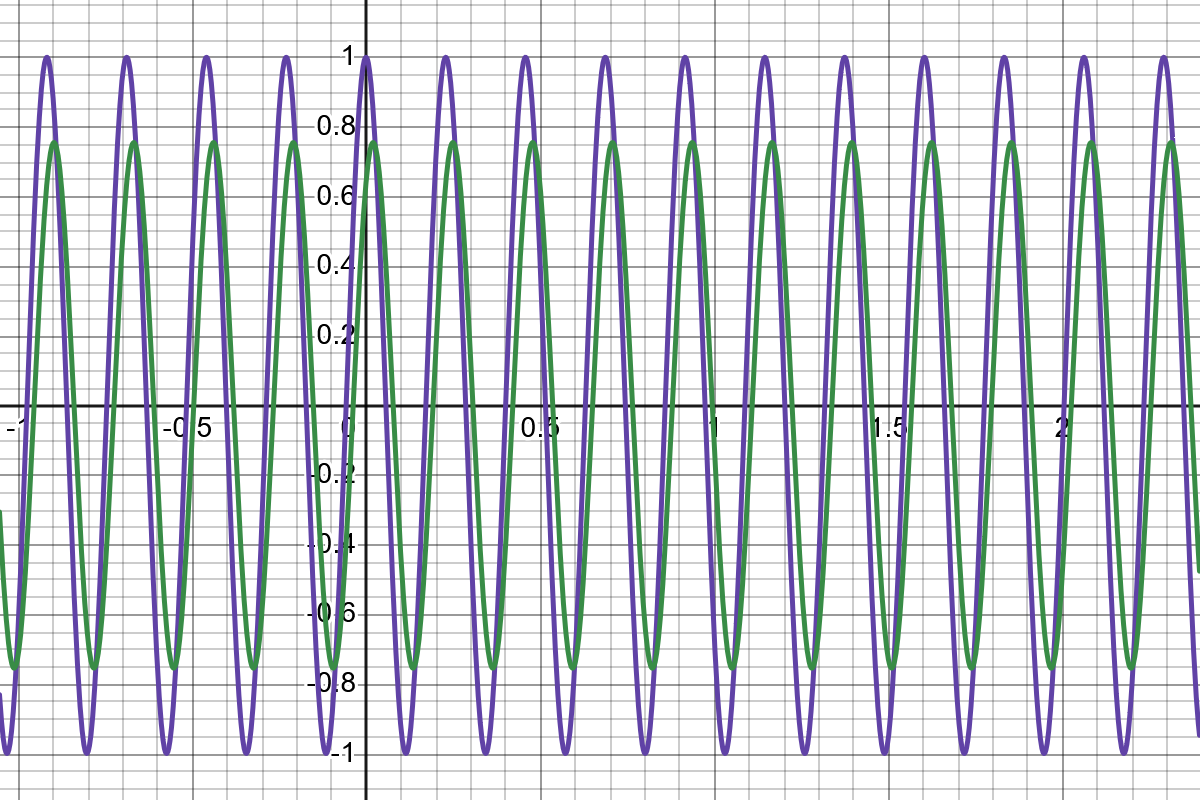
\includegraphics[scale=0.25]{rgadicoas/grafico3}
\end{table}

\newpage
\begin{center}
Gráfico 5: Tensão da fonte e $V_1$ em $\omega =2000\pi$
\end{center}

\vspace{30pt}
\begin{table}[h]
\centering
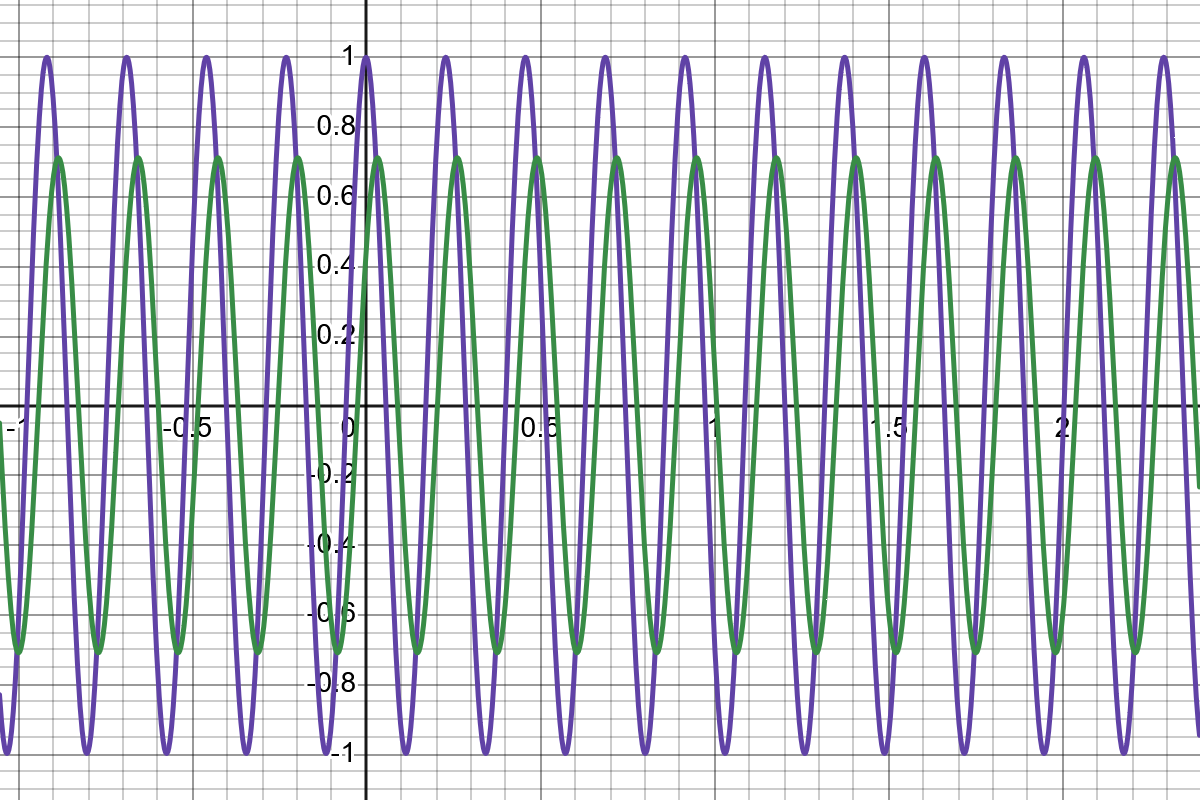
\includegraphics[scale=0.25]{rgadicoas/grafico7}
\end{table}

\begin{center}
Gráfico 6: Tensão da fonte e $V_2$ em $\omega =2000\pi$
\end{center}

\newpage
\begin{table}[h]
\centering
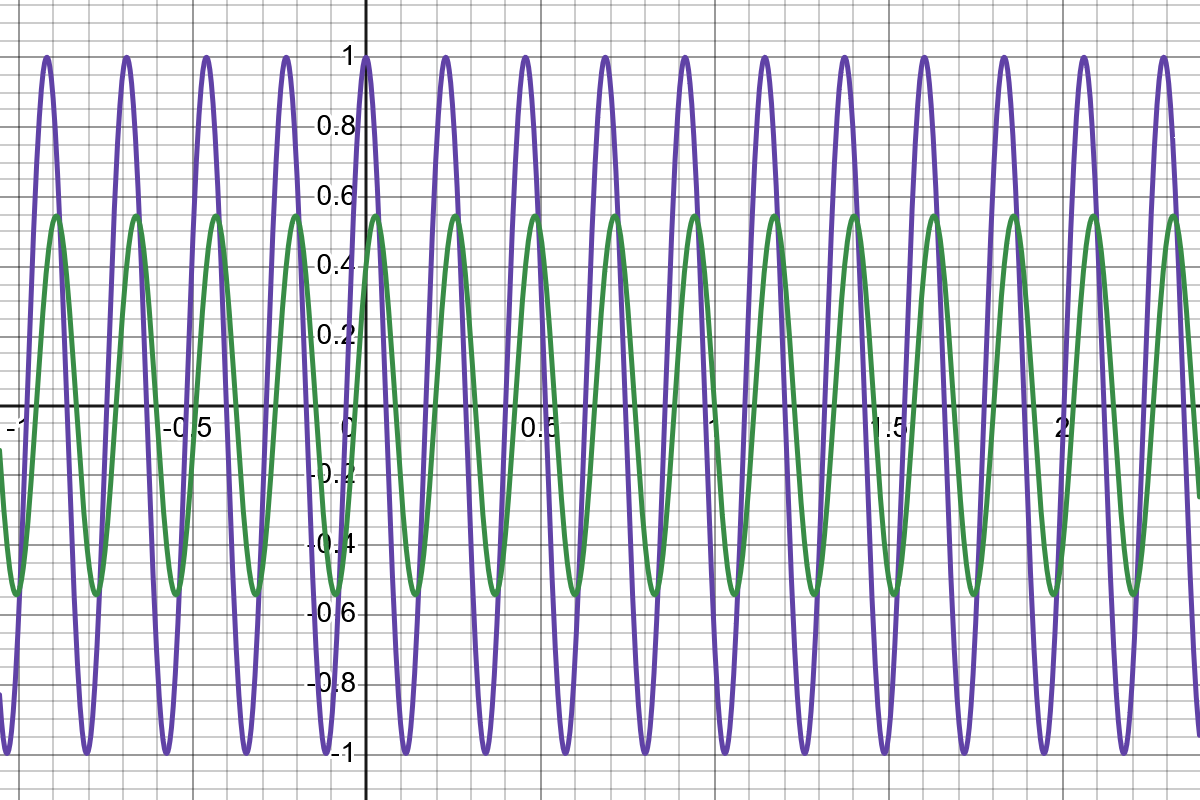
\includegraphics[scale=0.25]{rgadicoas/grafico4}
\end{table}

\begin{center}
Gráfico 7: Tensão da fonte e $V_1$ em $\omega =4000\pi$
\end{center}

\vspace{30pt}
\begin{table}[h]
\centering
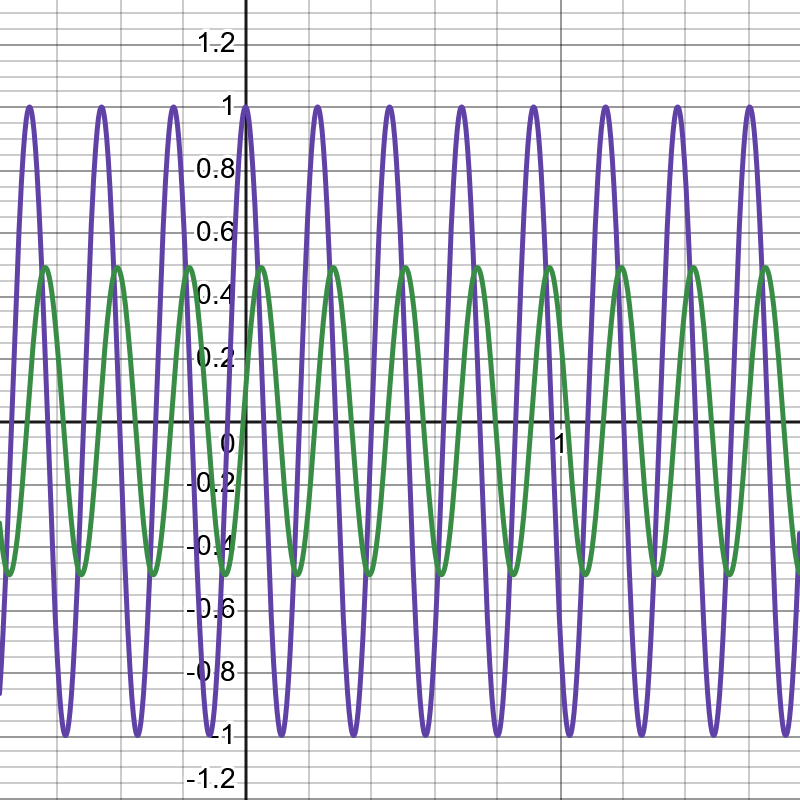
\includegraphics[scale=0.3]{rgadicoas/grafico8}
\end{table}

\begin{center}
Gráfico 8: Tensão da fonte e $V_2$ em $\omega =4000\pi$
\end{center}

\newpage
Tendo todos esses dados, foram feitas as medições no circuito físico, usando o osciloscópio do Elvis. Usando os cursores, são feitas as seguintes medições da amplitude das tensões e o dt (em segundos) entre os seus picos. O dt é então multiplicado pelo $\omega$ para descobrir a diferença de fase em radianos entre ambas as ondas, e esse valor é convertido para graus. 

\begin{table}[h]
\centering
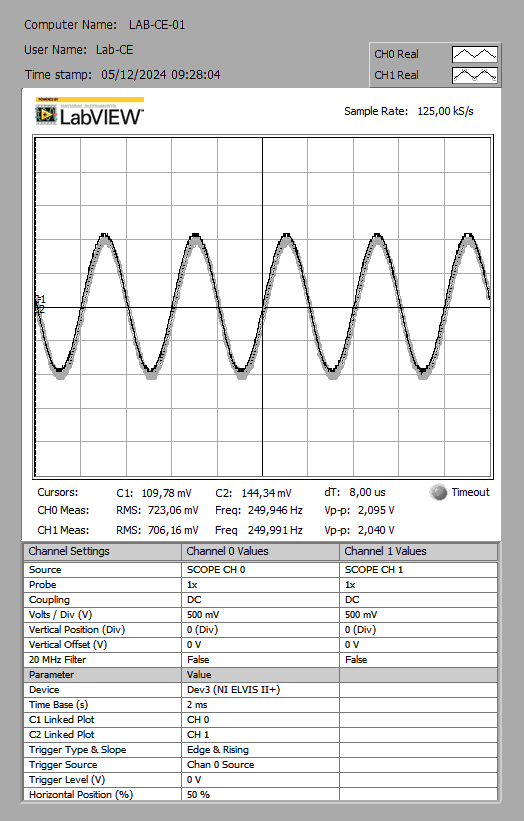
\includegraphics[scale=0.725]{rgadicoas/rgadicoa1}
\end{table}

\begin{center}
Gráfico 9: Tensão da fonte e $V_1$ em $f=250Hz$
\end{center}

\begin{table}[h]
\centering
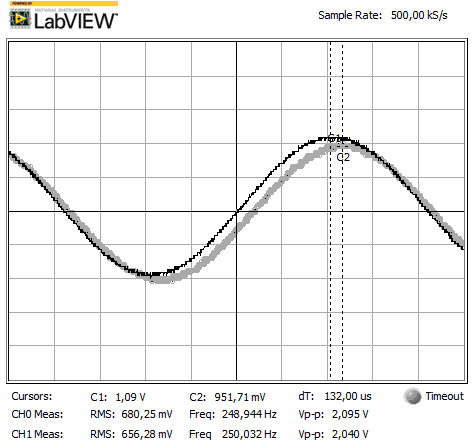
\includegraphics[scale=0.725]{rgadicoas/rgadicoa1-2}
\end{table}

\begin{center}
Gráfico 10: Tensão da fonte e $V_1$ em $f=250Hz$ (ampliado)
\end{center}

Amplitude $V_1$: $1,02V$, dt: $136\mu s\implies$ Fase $V_1$: $-12,26$\textdegree 

\newpage
\begin{table}[h]
\centering
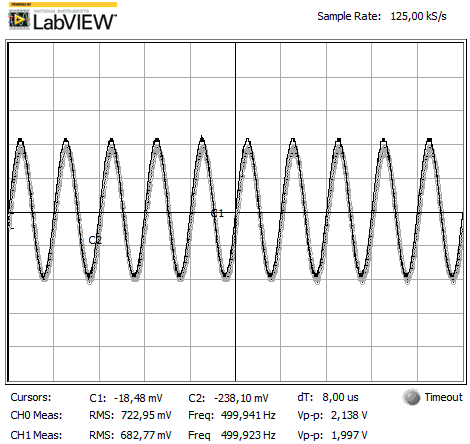
\includegraphics[scale=0.725]{rgadicoas/rgadicoa2}
\end{table}

\begin{center}
Gráfico 11: Tensão da fonte e $V_1$ em $f=500Hz$ 
\end{center}

\begin{table}[h]
\centering
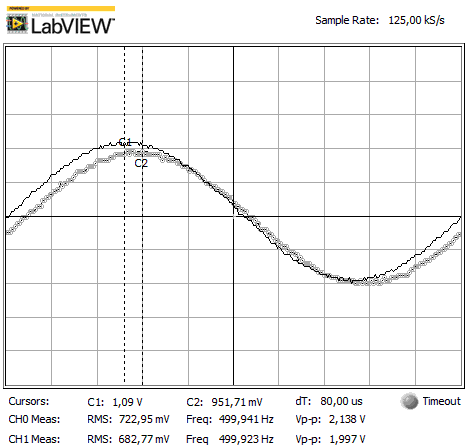
\includegraphics[scale=0.725]{rgadicoas/rgadicoa2-2}
\end{table}

\begin{center}
Gráfico 12: Tensão da fonte e $V_1$ em $f=500Hz$ (ampliado)
\end{center}

Amplitude $V_1$: $0,999V$, dt: $80\mu s\implies$ Fase $V_1$: $-14,38$\textdegree

\newpage
\begin{table}[h]
\centering
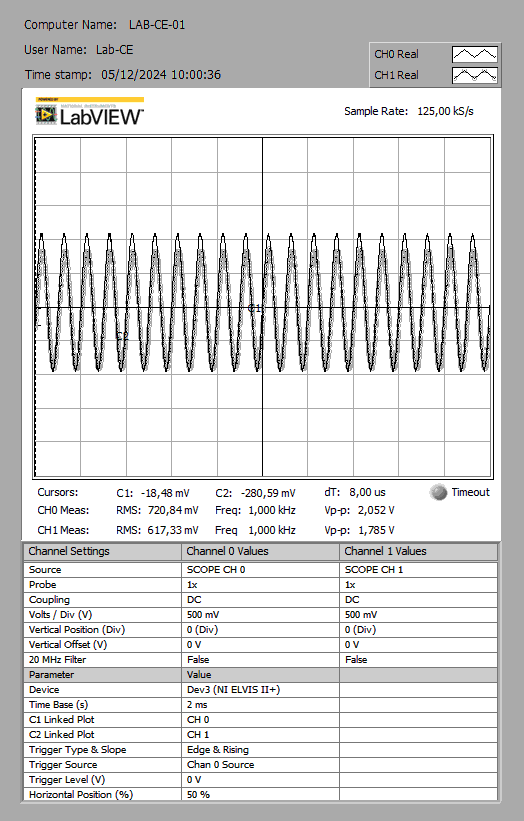
\includegraphics[scale=0.725]{rgadicoas/rgadicoa3}
\end{table}

\begin{center}
Gráfico 13: Tensão da fonte e $V_1$ em $f=1000Hz$ 
\end{center}

\begin{table}[h]
\centering
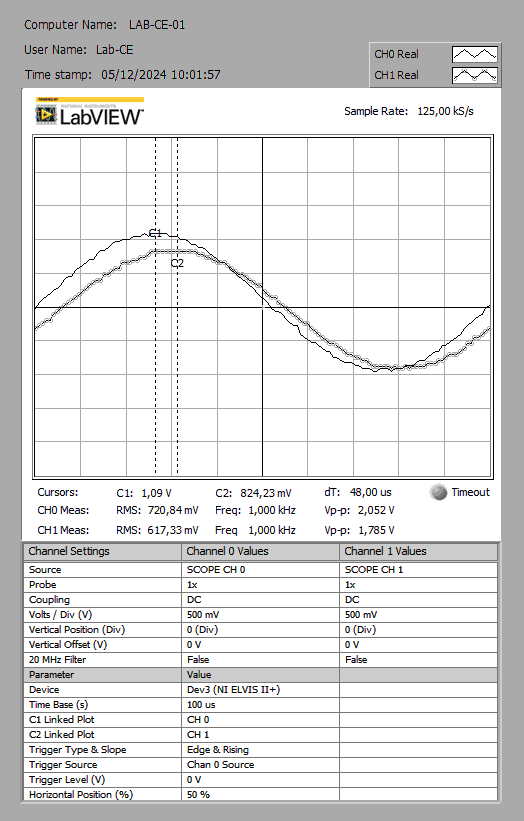
\includegraphics[scale=0.725]{rgadicoas/rgadicoa3-2}
\end{table}

\begin{center}
Gráfico 14: Tensão da fonte e $V_1$ em $f=1000Hz$ (ampliado)
\end{center}

Amplitude $V_1$: $0,893V$, dt: $48\mu s\implies$ Fase $V_1$: $-17,30$\textdegree

\newpage
\begin{table}[h]
\centering
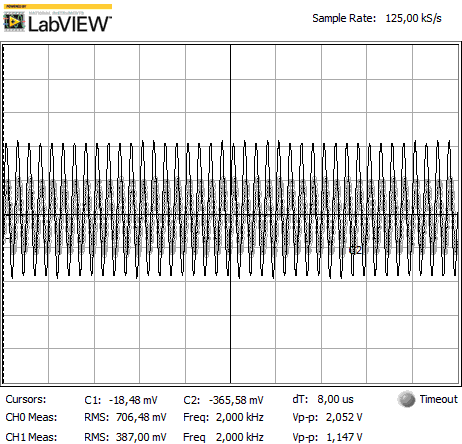
\includegraphics[scale=0.725]{rgadicoas/rgadicoa4}
\end{table}

\begin{center}
Gráfico 15: Tensão da fonte e $V_1$ em $f=2000Hz$ 
\end{center}

\begin{table}[h]
\centering
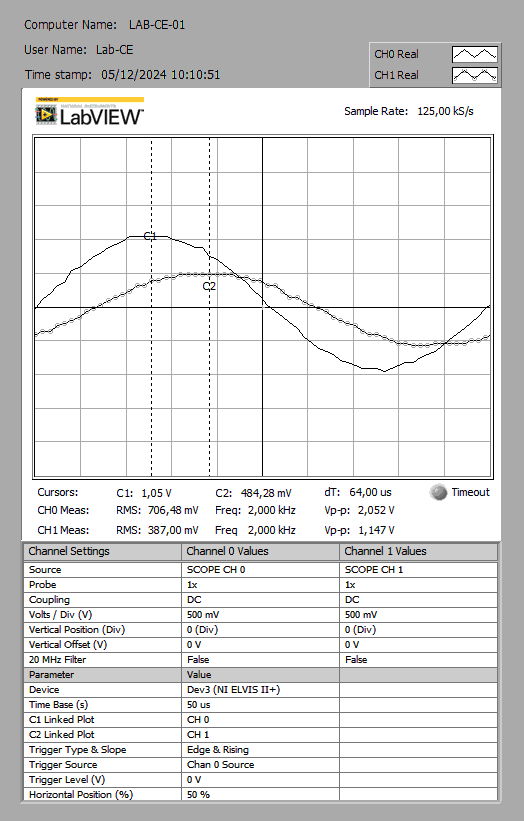
\includegraphics[scale=0.725]{rgadicoas/rgadicoa4-2}
\end{table}

\begin{center}
Gráfico 16: Tensão da fonte e $V_1$ em $f=2000Hz$ (ampliado)
\end{center}

Amplitude $V_1$: $0,574V$, dt: $64\mu s\implies$ Fase $V_1$: $-46,07$\textdegree

\newpage
\begin{table}[h]
\centering
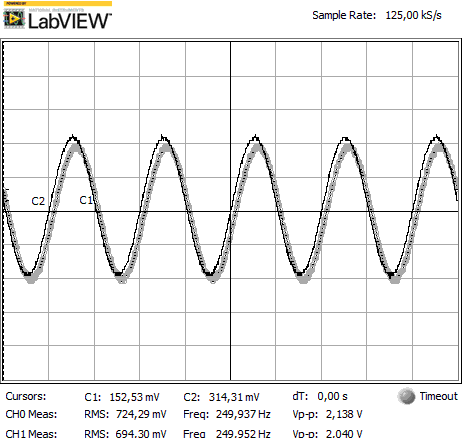
\includegraphics[scale=0.725]{rgadicoas/rgadicoa5}
\end{table}

\begin{center}
Gráfico 17: Tensão da fonte e $V_2$ em $f=250Hz$ 
\end{center}

\begin{table}[h]
\centering
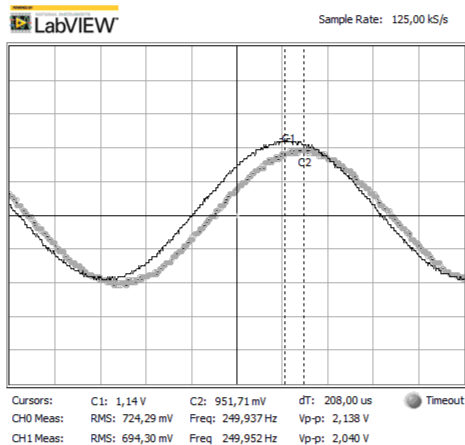
\includegraphics[scale=0.725]{rgadicoas/rgadicoa5-2}
\end{table}

\begin{center}
Gráfico 18: Tensão da fonte e $V_2$ em $f=250Hz$ (ampliado)
\end{center}

Amplitude $V_2$: $1,02V$, dt: $208\mu s\implies$ Fase $V_2$: $-18,74$\textdegree

\newpage
\begin{table}[h]
\centering
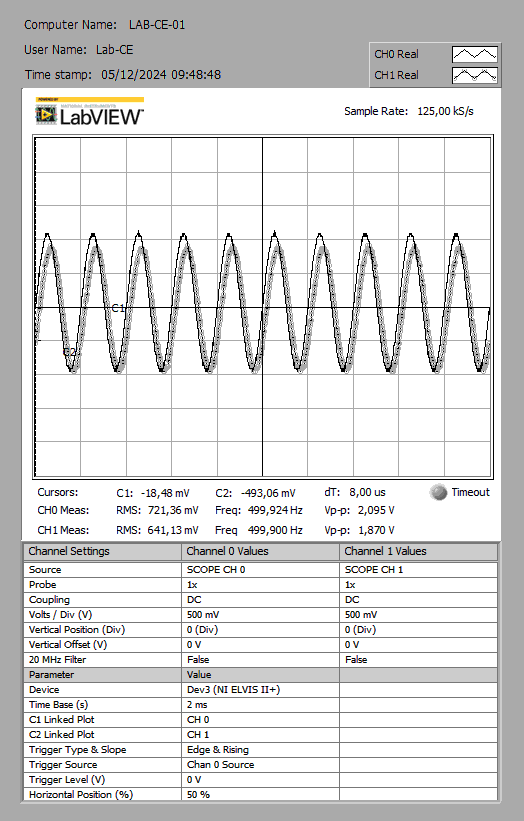
\includegraphics[scale=0.725]{rgadicoas/rgadicoa6}
\end{table}

\begin{center}
Gráfico 19: Tensão da fonte e $V_2$ em $f=500Hz$ 
\end{center}

\begin{table}[h]
\centering
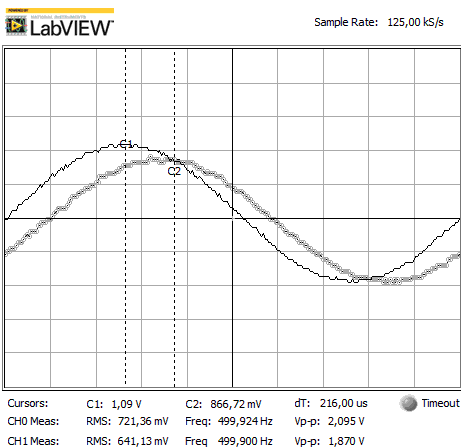
\includegraphics[scale=0.725]{rgadicoas/rgadicoa6-2}
\end{table}

\begin{center}
Gráfico 20: Tensão da fonte e $V_2$ em $f=500Hz$ (ampliado)
\end{center}

Amplitude $V_2$: $0,935V$, dt: $216\mu s\implies$ Fase $V_2$: $-38,90$\textdegree

\newpage
\begin{table}[h]
\centering
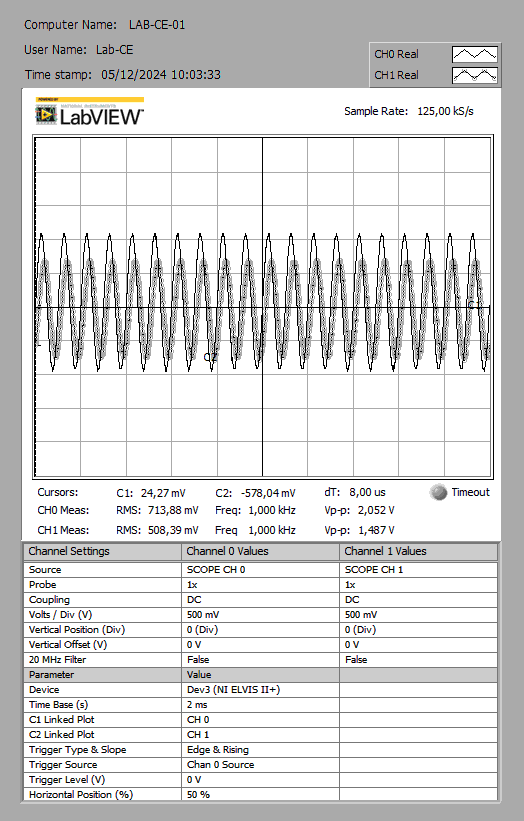
\includegraphics[scale=0.725]{rgadicoas/rgadicoa7}
\end{table}

\begin{center}
Gráfico 21: Tensão da fonte e $V_2$ em $f=1000Hz$ 
\end{center}

\begin{table}[h]
\centering
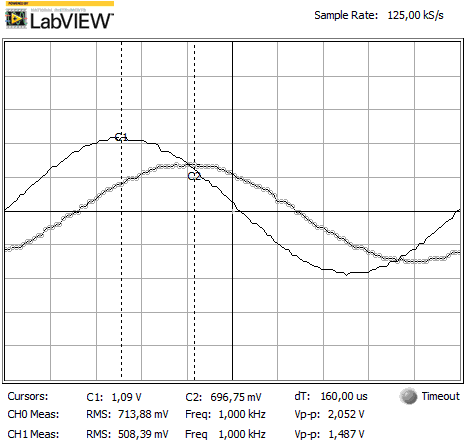
\includegraphics[scale=0.725]{rgadicoas/rgadicoa7-2}
\end{table}

\begin{center}
Gráfico 22: Tensão da fonte e $V_2$ em $f=1000Hz$ (ampliado)
\end{center}

Amplitude $V_2$: $0,744V$, dt: $160\mu s\implies$ Fase $V_2$: $-57,58$\textdegree

\newpage
\begin{table}[h]
\centering
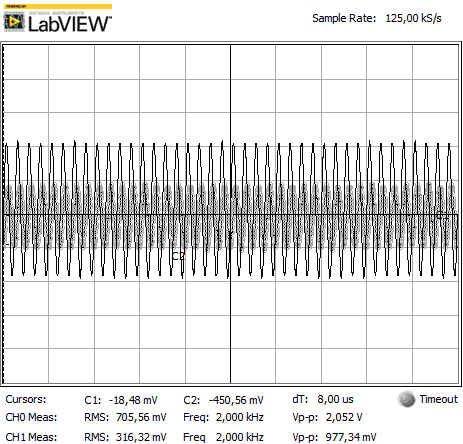
\includegraphics[scale=0.725]{rgadicoas/rgadicoa8}
\end{table}

\begin{center}
Gráfico 23: Tensão da fonte e $V_2$ em $f=2000Hz$ 
\end{center}

\begin{table}[h]
\centering
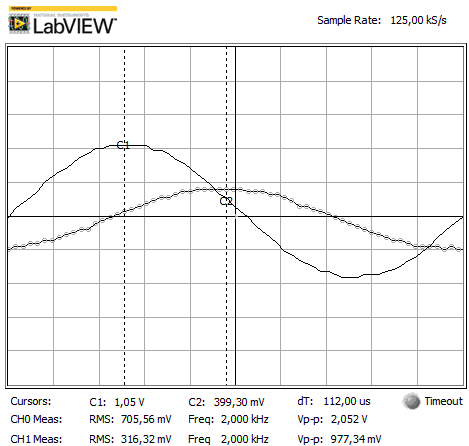
\includegraphics[scale=0.725]{rgadicoas/rgadicoa8-2}
\end{table}

\begin{center}
Gráfico 24: Tensão da fonte e $V_2$ em $f=2000Hz$ (ampliado)
\end{center}

Amplitude $V_2$: $0,489V$, dt: $112\mu s\implies$ Fase $V_2$: $-80,62$\textdegree

\newpage
Agora que temos todos os dados, montam-se as tabelas 2 e 3.

\vspace{5pt}
\begin{table}[h]
\centering
\begin{tabular}{|c|c|c|c|}
\hline
\textbf{Grandeza} & \textbf{Valor calculado} & \textbf{Valor medido} & \textbf{Erro (\%) }\\\hline
Amplitude de $V_1$ (frequência $0,25kHz$) & 0,975V & 1,02V & 4,62 \\\hline
Amplitude de $V_1$ (frequência $0,5kHz$) & 0,910V & 0,999V & 9,78 \\\hline
Amplitude de $V_1$ (frequência $1kHz$) & 0,755V & 0,893V & 18,28 \\\hline
Amplitude de $V_1$ (frequência $2kHz$) & 0,544V & 0,574V & 5,51 \\\hline
Fase de $V_1$ em relação a $V_0$ (frequência $0,25kHz$) & -10,34\textdegree & -12,26\textdegree & 18,57\\\hline
Fase de $V_1$ em relação a $V_0$ (frequência $0,5kHz$) & -19,25\textdegree & -14,38\textdegree & 25,30\\\hline
Fase de $V_1$ em relação a $V_0$ (frequência $1kHz$) & -32,24\textdegree & -17,30\textdegree & 46,34\\\hline
Fase de $V_1$ em relação a $V_0$ (frequência $2kHz$) & -42,47\textdegree & -46,07\textdegree & 8,48\\\hline
\end{tabular}
\caption*{Tabela 2: Tensões no capacitor $C_1$}
\end{table}
\vspace{5pt}
\begin{table}[h]
\centering
\begin{tabular}{|c|c|c|c|}
\hline
\textbf{Grandeza} & \textbf{Valor nominal} & \textbf{Valor medido} & \textbf{Erro (\%) }\\\hline
Amplitude de $V_2$ (frequência $0,25kHz$) & 0,972V & 1,02V & 4,94 \\\hline
Amplitude de $V_2$ (frequência $0,5kHz$) & 0,897V & 0,935V & 4,24 \\\hline
Amplitude de $V_2$ (frequência $1kHz$) & 0,711V & 0,744V & 4,64 \\\hline
Amplitude de $V_2$ (frequência $2kHz$) & 0,441V & 0,489V & 10,88 \\\hline
Fase de $V_2$ em relação a $V_0$ (frequência $0,25kHz$) & -15,45\textdegree & -18,74\textdegree & 21,29\\\hline
Fase de $V_2$ em relação a $V_0$ (frequência $0,5kHz$) & -29,88\textdegree & -38,90\textdegree & 30,19\\\hline
Fase de $V_2$ em relação a $V_0$ (frequência $1kHz$) & -52,08\textdegree & -57,58\textdegree & 10,56\\\hline
Fase de $V_2$ em relação a $V_0$ (frequência $2kHz$) & -78,36\textdegree & -80,62\textdegree & 2,88\\\hline
\end{tabular}
\caption*{Tabela 3: Tensão no capacitor $C_2$}
\end{table}




\newpage
\section{Conclusão}

\section{Bibliografia}

\end{document}